\documentclass[11pt,a4paper]{article}

\usepackage[margin=1in]{geometry}
\usepackage{graphicx}
\usepackage{booktabs}
\usepackage{array}
\usepackage{float}
\usepackage{url}
\usepackage{amsmath}
\usepackage{tikz}
\usetikzlibrary{positioning,arrows.meta}
\usepackage[hidelinks]{hyperref}

\graphicspath{{figures/}}
\setlength{\emergencystretch}{3em}   % avoid overfull lines with long paths / arrows

\title{\textbf{SentiBias Audit}\\[4pt]
\large Auditing Multilingual Sentiment Models for Dialect, Gender and Code-Switching Bias\\[6pt]
\normalsize AI Project --- Final Technical Report (Deliverable 3, Track B: Research)}
\author{Saad Jahangir \and Talmeez ur Rehman \and Muhammad Yaseen Asif}
\date{November 2026}

\begin{document}
\maketitle

\begin{abstract}
Sentiment models are usually evaluated on standard English, but they are deployed for users
who write in other language varieties. SentiBias Audit tests whether a multilingual sentiment
pipeline is equally reliable for English, Roman Urdu and code-switched Roman Urdu--English
text, and for sentences that differ only in a gender- or race-coded name. We collected and
cleaned three public datasets (UCI Roman Urdu, TweetEval, Equity Evaluation Corpus; 87,696
rows), embedded all text with a frozen multilingual MiniLM transformer, and trained a PyTorch
MLP head (tuned with a 24-configuration grid search) against a TF-IDF + Logistic Regression
baseline. On a held-out stratified test split the model reaches a macro-F1 of 0.638 and an
AUC-ROC of 0.828 (baseline 0.616 / 0.806), a statistically significant improvement overall
(McNemar $p = 2\times10^{-5}$), but it is significantly \emph{worse} than the baseline on
Roman Urdu (0.535 vs.\ 0.573), so the English--Roman Urdu gap grows from 0.056 to 0.136. A
3-seed ablation study shows why: the pre-trained representation is the most important component
on English ($-0.105$ macro-F1 without it) but contributes nothing on Roman Urdu, where only Roman
Urdu training data and the non-linear head carry the performance. On the EEC the model shows a
small but significant gender gap. Language re-weighting reduced the language gap by 14\%, while
counterfactual gender augmentation did not reduce the gender gap of the frozen encoder. We
discuss why samples fail (neutral boundary, Roman Urdu representation, negation, sarcasm, 8.8\%
label conflicts) and the limits of a frozen-encoder approach.
\end{abstract}

\tableofcontents
\newpage

% ===========================================================================
\section{Introduction}
Sentiment analysis models are used for content moderation, brand monitoring and customer
support triage, but they are mostly trained and evaluated on standard English. SentiBias
Audit asks whether a widely used multilingual sentiment pipeline is \emph{equally reliable}
for three groups that are under-represented in that setting: users who write in Roman Urdu,
users who mix Roman Urdu and English in one sentence (code-switching), and people referred
to by female or male (and African-American or European) names.

The project ran in six phases over three deliverables. Deliverable~1 defined the problem
(Phase~1) and built the data pipeline (Phase~2). Deliverable~2 built and evaluated the models
(Phases~3 and~4). This final report merges both and adds Phase~5 (comparative analysis,
ablation study, bias mitigation and result discussion) and Phase~6 (this document). All code
is in the GitHub repository \url{https://github.com/Sed-J05/SentiBias-Audit}:
\path{data_scripts/} for Phase~2 and \path{src/} for Phases~3--5.

% ===========================================================================
\section{Phase 1: Problem Definition}

\subsection{Problem Statement}
Two groups are especially affected in Pakistan and the South-Asian diaspora:
\begin{itemize}
  \item \textbf{Roman Urdu and code-switched writers.} Much informal online Urdu is written in
        Latin script (``Roman Urdu'') with no standard spelling (\emph{nahi / nhi / nahin})
        and is often mixed with English words in one sentence. Models that have rarely seen
        this variety tend to default to \emph{neutral} or give unstable predictions, so the
        opinions of these users are systematically mis-measured.
  \item \textbf{People referred to by gender- or race-coded names.} Kiritchenko and
        Mohammad~\cite{eec} showed that many sentiment systems give different scores to two
        sentences that differ only in a first name (\emph{``Amanda feels angry''} vs.\
        \emph{``Alonzo feels angry''}). Such differences are not caused by the meaning of the
        text and are an unfair, measurable bias.
\end{itemize}
The pain point is that a model can be \emph{accurate on average} while being
\emph{unreliable for specific language varieties and demographic groups}. These gaps are
invisible in a single accuracy number. SentiBias Audit measures them for a multilingual
transformer pipeline and tests whether standard mitigation methods (re-weighting,
counterfactual data augmentation) reduce them.

\subsection{Target Audience}
\begin{itemize}
  \item \textbf{Research gap.} Bias audits of sentiment analysis exist for English gender and
        race (EEC) and for some high-resource languages, but there is no audit that combines
        Roman Urdu, Roman Urdu--English code-switching and gender-coded names, and evaluates
        mitigation on all of them.
  \item \textbf{Practitioners} in Pakistan who deploy off-the-shelf multilingual sentiment
        models and need to know \emph{where} a model fails before trusting it.
  \item \textbf{Fairness researchers and educators} who need a reproducible pipeline and a
        cleaned evaluation set for South-Asian code-switched text.
\end{itemize}

\subsection{AI Justification}
A rule-based or lexicon-based approach is not viable: (1)~Roman Urdu has an open vocabulary
with no spelling standard, so a lexicon cannot list all variants, while sub-word tokenisation
and learned embeddings generalise across spellings; (2)~polarity depends on context
(\emph{``bilkul bhi acha nahi''} = not good at all), which needs learned representations;
(3)~code-switching can change language at any token, which a multilingual model handles
natively; (4)~the object of study is itself a learned model, and the bias we audit comes from
statistical patterns in training data, so measuring and reducing it is a machine-learning
problem.

% ===========================================================================
\section{Phase 2: Data Acquisition \& Preprocessing}

\subsection{Collection}
Three public datasets were selected, one per bias dimension (Table~\ref{tab:datasets}).
\path{data_scripts/download_data.py} downloads every file with \texttt{requests}, unzips the
EEC archive and writes one log line per file (timestamp, HTTP status, bytes, URL) to
\path{data/raw/download_log.txt}. Raw data is git-ignored; the EEC licence forbids
redistribution, so it is always fetched from the original page.

\begin{table}[H]
\centering
\footnotesize
\begin{tabular}{llrl}
\toprule
\textbf{Dataset} & \textbf{Bias dimension} & \textbf{Raw rows} & \textbf{Source} \\
\midrule
Roman Urdu Data Set~\cite{uci} & Roman Urdu, code-switching & 20,229 & UCI ML Repository \#458 \\
TweetEval Sentiment~\cite{tweeteval} & English reference (tweets) & 59,899 & Cardiff NLP, GitHub \\
Equity Evaluation Corpus~\cite{eec} & Gender- and race-coded names & 8,640 & Kiritchenko \& Mohammad \\
\bottomrule
\end{tabular}
\caption{Datasets used in the project.}
\label{tab:datasets}
\end{table}

\subsection{Cleaning}
\path{data_scripts/clean_data.py} applies three steps to every dataset and writes one tidy CSV
per dataset plus a combined master file with a unified schema (\texttt{text, label, language,
source, split, gender, code\_switched, n\_tokens, n\_chars, english\_word\_ratio}).
\begin{enumerate}
  \item \textbf{Missing values.} Rows without text or label are dropped and whitespace is
        normalised. The junk third column of the Roman Urdu file is removed and the typo label
        \texttt{Neative} is corrected. Missing EEC \texttt{Race}/\texttt{Emotion} cells are
        meaningful (noun-phrase rows, neutral templates), so they are imputed with
        \texttt{none}; EEC emotions are mapped to labels (joy $\to$ positive; anger, sadness,
        fear $\to$ negative; none $\to$ neutral).
  \item \textbf{Duplicates.} Exact duplicate texts are removed (first occurrence kept).
  \item \textbf{Outliers.} Rows above Tukey's outer fence $Q_3 + 3\,\mathrm{IQR}$ on token
        count (50 tokens for Roman Urdu, 43 for TweetEval) are removed.
\end{enumerate}
A lexicon heuristic flags a Roman Urdu sample as \textbf{code-switched} if it contains at least
two unambiguous English words; 959 samples (5.0\%) are flagged.

\begin{table}[H]
\centering
\small
\begin{tabular}{lrrrr}
\toprule
\textbf{Dataset} & \textbf{Raw} & \textbf{After missing} & \textbf{After duplicates} & \textbf{After outliers} \\
\midrule
Roman Urdu & 20,229 & 20,116 & 19,582 & 19,187 \\
TweetEval  & 59,899 & 59,899 & 59,869 & 59,869 \\
EEC        & 8,640  & 8,640  & 8,640  & 8,640 \\
\midrule
\textbf{Master} & 88,768 & & & \textbf{87,696} \\
\bottomrule
\end{tabular}
\caption{Row counts after each cleaning step.}
\label{tab:cleaning}
\end{table}

\subsection{Feature Strategy}
\path{data_scripts/feature_eda.py} normalises the text (lowercase, URL/mention/number
placeholders, punctuation removed), label-encodes the target (negative~=~0, neutral~=~1,
positive~=~2), one-hot encodes language and gender, builds a TF-IDF matrix (unigrams +
bigrams, 5,000 features, \texttt{min\_df}=2) and scales the numeric features with z-score and
min--max scaling. The normalised text feeds the TF-IDF baseline; the transformer model uses
the raw text, because its tokenizer handles casing and punctuation itself.

\subsection{Exploratory Data Analysis}
\begin{figure}[H]
\centering
\begin{minipage}{0.49\textwidth}
  \centering
  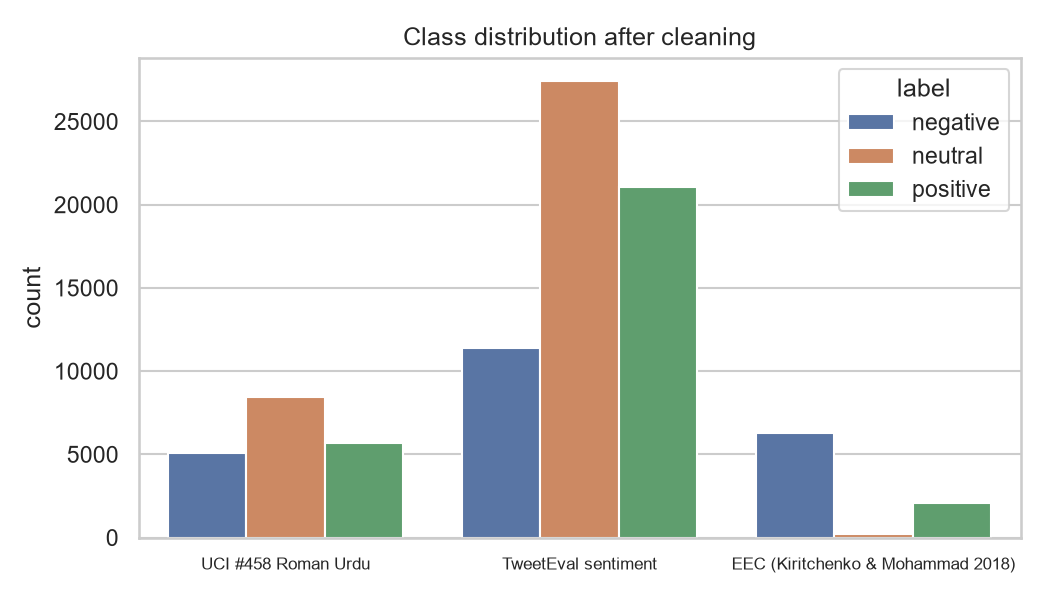
\includegraphics[width=\textwidth]{clean_class_distribution.png}
\end{minipage}\hfill
\begin{minipage}{0.49\textwidth}
  \centering
  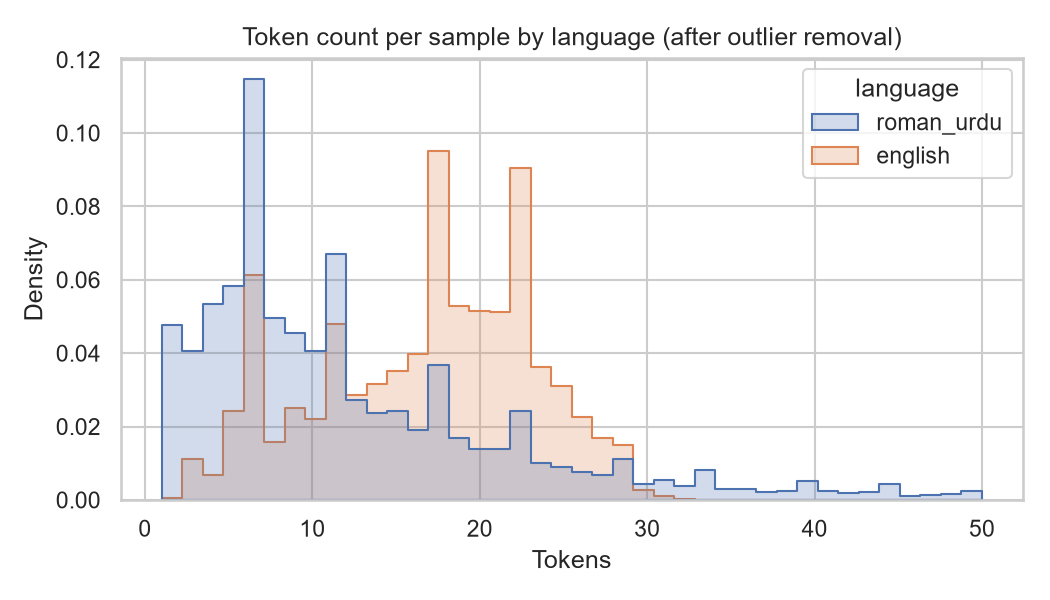
\includegraphics[width=\textwidth]{text_length_distribution.png}
\end{minipage}
\caption{Left: class distribution per source after cleaning. Neutral dominates both training
corpora; EEC is negative-heavy by construction. Right: Roman Urdu samples are much shorter
(median 9 tokens) than English tweets (18--23 tokens).}
\label{fig:eda1}
\end{figure}

\begin{figure}[H]
\centering
\begin{minipage}{0.49\textwidth}
  \centering
  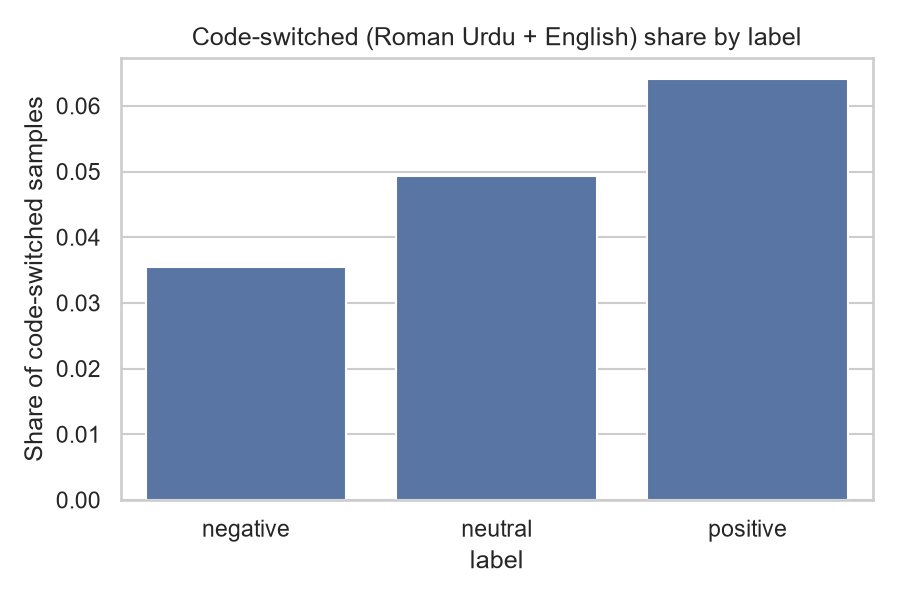
\includegraphics[width=\textwidth]{code_switching_by_label.png}
\end{minipage}\hfill
\begin{minipage}{0.49\textwidth}
  \centering
  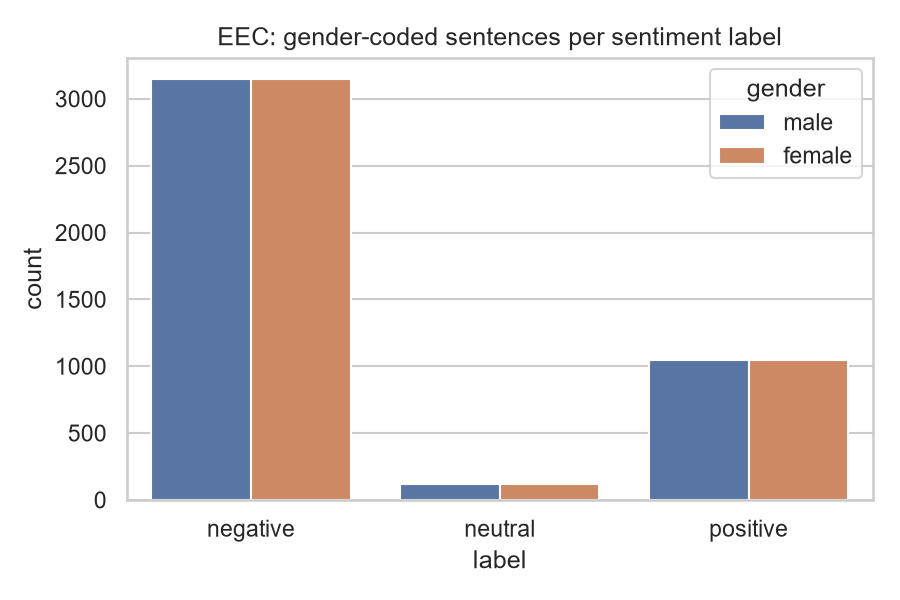
\includegraphics[width=\textwidth]{eec_gender_balance.png}
\end{minipage}
\caption{Left: positive Roman Urdu samples switch to English almost twice as often as negative
ones (6.4\% vs.\ 3.5\%). Right: EEC is exactly balanced between female and male within every
label, which makes paired counterfactual evaluation possible.}
\label{fig:eda2}
\end{figure}

% ===========================================================================
\section{Phase 3: Model Architecture \& Implementation}

\subsection{Framework Selection}
\textbf{PyTorch}~\cite{pytorch} is used for the main model (layers, loss, optimizer and training
loop are written by hand in \path{src/model.py} and \path{src/train.py});
\textbf{sentence-transformers} loads the pre-trained encoder
\texttt{paraphrase-multilingual-MiniLM-L12-v2}~\cite{sbert,sbertmulti,minilm}, trained on 50+
languages including Urdu; \textbf{scikit-learn}~\cite{sklearn} is used for the baseline, the
split and all metrics. The encoder is \emph{frozen}: all 87,696 sentences are embedded once
(\path{src/embed.py}, 23~minutes on a 12-core CPU, no GPU) and only the classification head is
trained. This made a full hyperparameter grid, a 3-seed ablation study and several mitigation
runs possible on a laptop. It also matches the audit goal: we measure the bias of a widely
used pre-trained encoder, not of weights we changed ourselves.

\subsection{Design: Layers, Loss and Optimizer}
\begin{figure}[H]
\centering
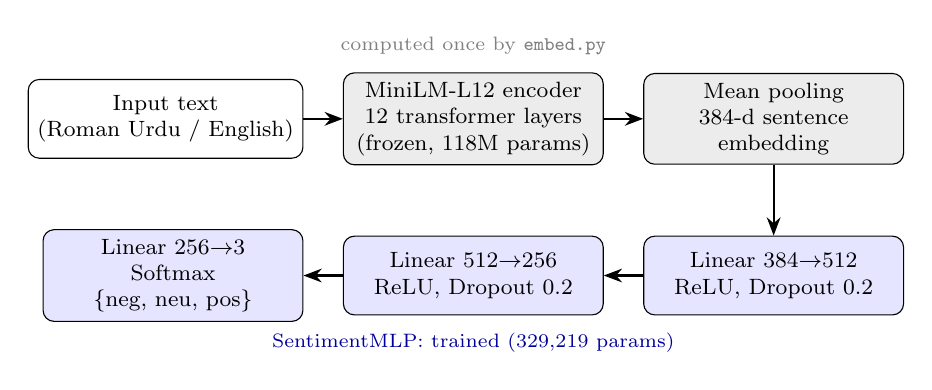
\begin{tikzpicture}[
  node distance=5mm,
  box/.style={draw, rounded corners, align=center, minimum width=3.3cm, minimum height=10mm, font=\footnotesize},
  frozen/.style={box, fill=gray!15},
  train/.style={box, fill=blue!10},
  arr/.style={-{Stealth}, thick}]
\node[box] (in) {Input text\\(Roman Urdu / English)};
\node[frozen, right=of in] (enc) {MiniLM-L12 encoder\\12 transformer layers\\(frozen, 118M params)};
\node[frozen, right=of enc] (pool) {Mean pooling\\384-d sentence\\embedding};
\node[train, below=9mm of pool] (l1) {Linear 384$\to$512\\ReLU, Dropout 0.2};
\node[train, left=of l1] (l2) {Linear 512$\to$256\\ReLU, Dropout 0.2};
\node[train, left=of l2] (l3) {Linear 256$\to$3\\Softmax\\\{neg, neu, pos\}};
\draw[arr] (in) -- (enc); \draw[arr] (enc) -- (pool); \draw[arr] (pool) -- (l1);
\draw[arr] (l1) -- (l2); \draw[arr] (l2) -- (l3);
\node[font=\scriptsize, gray, above=1mm of enc] {computed once by \texttt{embed.py}};
\node[font=\scriptsize, blue!60!black, below=1mm of l2] {SentimentMLP: trained (329,219 params)};
\end{tikzpicture}
\caption{Architecture of the main model. Grey: frozen pre-trained encoder. Blue: trainable
classification head \texttt{SentimentMLP} with the tuned sizes $h = 512$, $p = 0.2$.}
\label{fig:arch}
\end{figure}

\paragraph{Layers.} \texttt{SentimentMLP} is a two-hidden-layer perceptron:
\[
\begin{aligned}
&\text{Linear}(384, h) \to \text{ReLU} \to \text{Dropout}(p) \to \text{Linear}(h, h/2)\\
&\quad\to \text{ReLU} \to \text{Dropout}(p) \to \text{Linear}(h/2, 3).
\end{aligned}
\]

\paragraph{Loss function.} The training data is imbalanced (neutral 45\%, positive 34\%,
negative 21\%), so we use class-weighted cross-entropy
\[
\mathcal{L} = -\frac{1}{N}\sum_{i} w_{y_i}\log \operatorname{softmax}(z_i)_{y_i},\qquad
w_c = \frac{N}{3\,N_c},
\]
which gives $w_{\text{neg}} = 1.60$, $w_{\text{neu}} = 0.73$, $w_{\text{pos}} = 0.99$.

\paragraph{Optimizer.} AdamW~\cite{adamw} with weight decay $10^{-4}$, shuffled mini-batches,
at most 40 epochs, and early stopping on validation macro-F1 (patience~4, best weights
restored).

\paragraph{Baseline.} \path{src/baseline.py}: TF-IDF (same settings as Phase~2, but the
vocabulary is now fitted on the training split only to avoid leakage) followed by multinomial
Logistic Regression with balanced class weights. A majority-class predictor is added as a
trivial lower bound in Phase~5.

\subsection{Hyperparameter Tuning}
\path{src/tune.py} runs a full grid of $3 \times 2 \times 2 \times 2 = 24$ configurations, each
trained with early stopping and scored by validation macro-F1 (the test split is never used
for tuning).

\begin{table}[H]
\centering
\small
\begin{tabular}{lll}
\toprule
\textbf{Hyperparameter} & \textbf{Values tested} & \textbf{Selected} \\
\midrule
Learning rate (AdamW) & $10^{-2}$, $10^{-3}$, $10^{-4}$ & $10^{-4}$ \\
Batch size            & 64, 256                         & 64 \\
Dropout $p$           & 0.2, 0.5                        & 0.2 \\
Hidden size $h$       & 256, 512                        & 512 \\
Weight decay          & $10^{-4}$ (fixed)               & $10^{-4}$ \\
Epochs                & early stopping, patience 4      & 11 (best epoch) \\
\midrule
Baseline: LogReg $C$  & 0.1, 0.3, 1, 3, 10              & 1 \\
\bottomrule
\end{tabular}
\caption{Search space and final selection. Best validation macro-F1: 0.646 (MLP), 0.618
(baseline). Full results: \texttt{results/tuning\_results.csv}, \texttt{results/baseline\_tuning.csv}.}
\label{tab:grid}
\end{table}

The learning rate matters most: with $10^{-2}$ training is unstable (worst run 0.50
macro-F1), $10^{-3}$ overfits after a few epochs, and $10^{-4}$ gives the best 4 of 24 runs.
Batch size 64 is slightly better than 256 and needs half the epochs. Dropout 0.2 beats 0.5
because the input is already a compact pre-trained embedding, and hidden size 512 beats 256 in
every pair at $10^{-4}$. Retraining with the selected values reproduces the tuning score
exactly (0.6462, fixed seed 42).

% ===========================================================================
\section{Phase 4: Training \& Evaluation}

\subsection{Validation Strategy}
\path{src/split_data.py} creates one fixed \textbf{stratified 70/15/15 split} of the two
labelled corpora, stratified by \emph{language $\times$ label} (train / val / test = 55,339 /
11,858 / 11,859 rows; Roman Urdu is 24\% of every split). The \textbf{EEC is never used for
training}: all 8,640 EEC sentences form a separate ``bias'' split used only for the Bias Check.
Validation is used for early stopping, tuning and model selection; the test split is used only
for the final numbers.

\subsection{Training History}
\begin{figure}[H]
\centering
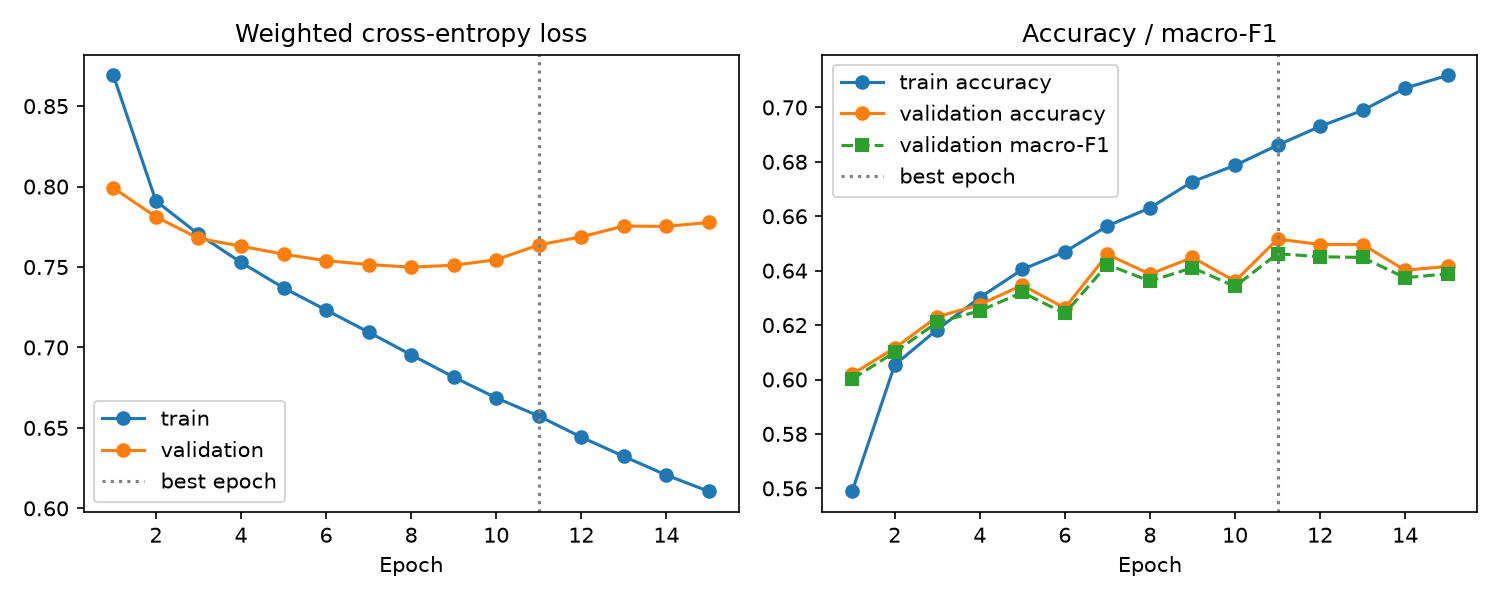
\includegraphics[width=0.92\textwidth]{training_curves.png}
\caption{Training history of the final model. Training loss keeps falling, but validation
macro-F1 peaks at epoch~11; early stopping ended training at epoch~15 and restored the
epoch-11 weights.}
\label{fig:curves}
\end{figure}

\subsection{Metric Analysis}
\textbf{Macro-F1 is the main metric} (model selection and early stopping): the classes are
imbalanced and macro-averaging gives the small negative class the same weight as neutral.
Precision and recall are reported separately because false alarms (neutral flagged as
negative) and missed negatives cost different things. AUC-ROC (one-vs-rest, macro) measures
ranking quality independently of the threshold and the class priors, which differ between the
corpora. Accuracy is reported only for completeness.

\begin{table}[H]
\centering
\small
\begin{tabular}{lrrrrr}
\toprule
\textbf{Model} & \textbf{Accuracy} & \textbf{Macro-P} & \textbf{Macro-R} & \textbf{Macro-F1} & \textbf{Macro AUC} \\
\midrule
TF-IDF + LogReg (baseline) & 0.621 & 0.612 & 0.633 & 0.616 & 0.806 \\
MiniLM + MLP (ours)        & \textbf{0.643} & \textbf{0.633} & \textbf{0.652} & \textbf{0.638} & \textbf{0.828} \\
\bottomrule
\end{tabular}
\caption{Results on the held-out test split (11,859 rows).}
\label{tab:test}
\end{table}

\begin{table}[H]
\centering
\small
\begin{tabular}{lrrrrrrr}
\toprule
 & & \multicolumn{3}{c}{\textbf{TF-IDF + LogReg}} & \multicolumn{3}{c}{\textbf{MiniLM + MLP}} \\
\cmidrule(lr){3-5}\cmidrule(lr){6-8}
\textbf{Class} & \textbf{Support} & P & R & F1 & P & R & F1 \\
\midrule
Negative & 2,470 & 0.487 & 0.673 & 0.565 & 0.524 & 0.690 & 0.595 \\
Neutral  & 5,385 & 0.686 & 0.571 & 0.623 & 0.690 & 0.612 & 0.649 \\
Positive & 4,004 & 0.663 & 0.657 & 0.660 & 0.684 & 0.655 & 0.669 \\
\bottomrule
\end{tabular}
\caption{Per-class precision, recall and F1 on the test split.}
\label{tab:perclass}
\end{table}

\begin{figure}[H]
\centering
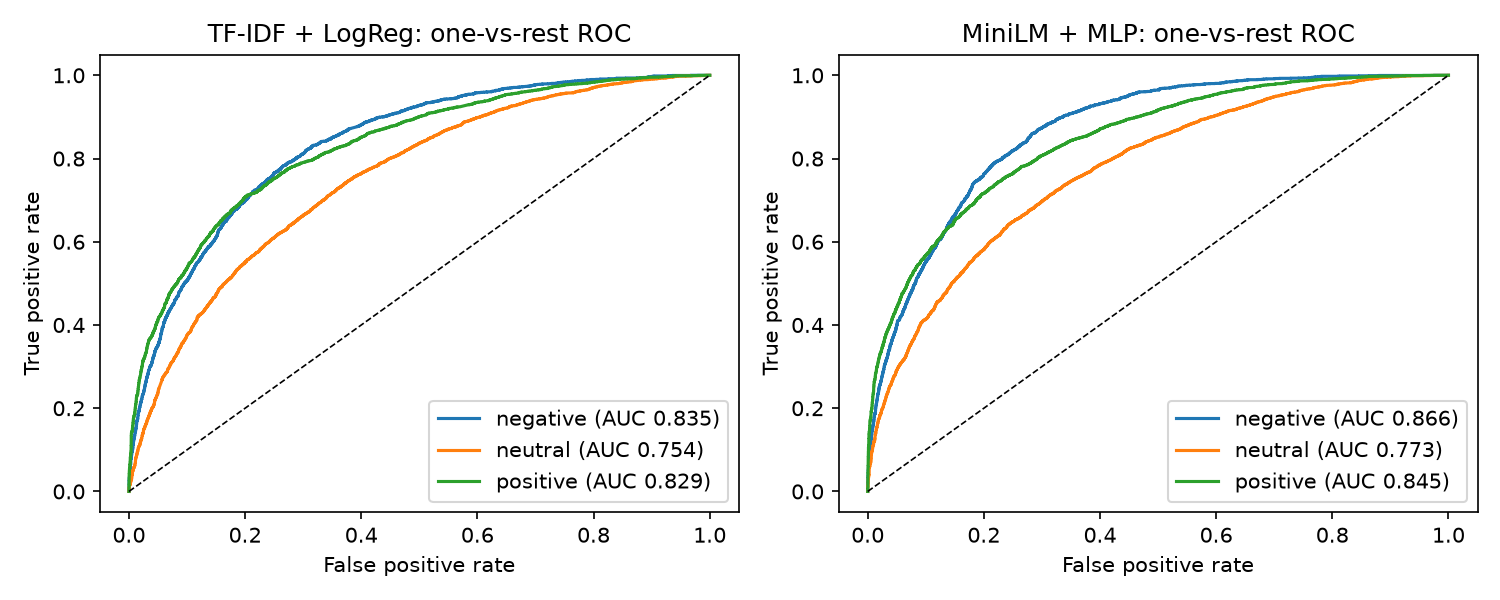
\includegraphics[width=0.92\textwidth]{roc_curves.png}
\caption{One-vs-rest ROC curves on the test split. Neutral is the hardest class for both models.}
\label{fig:roc}
\end{figure}

\begin{figure}[H]
\centering
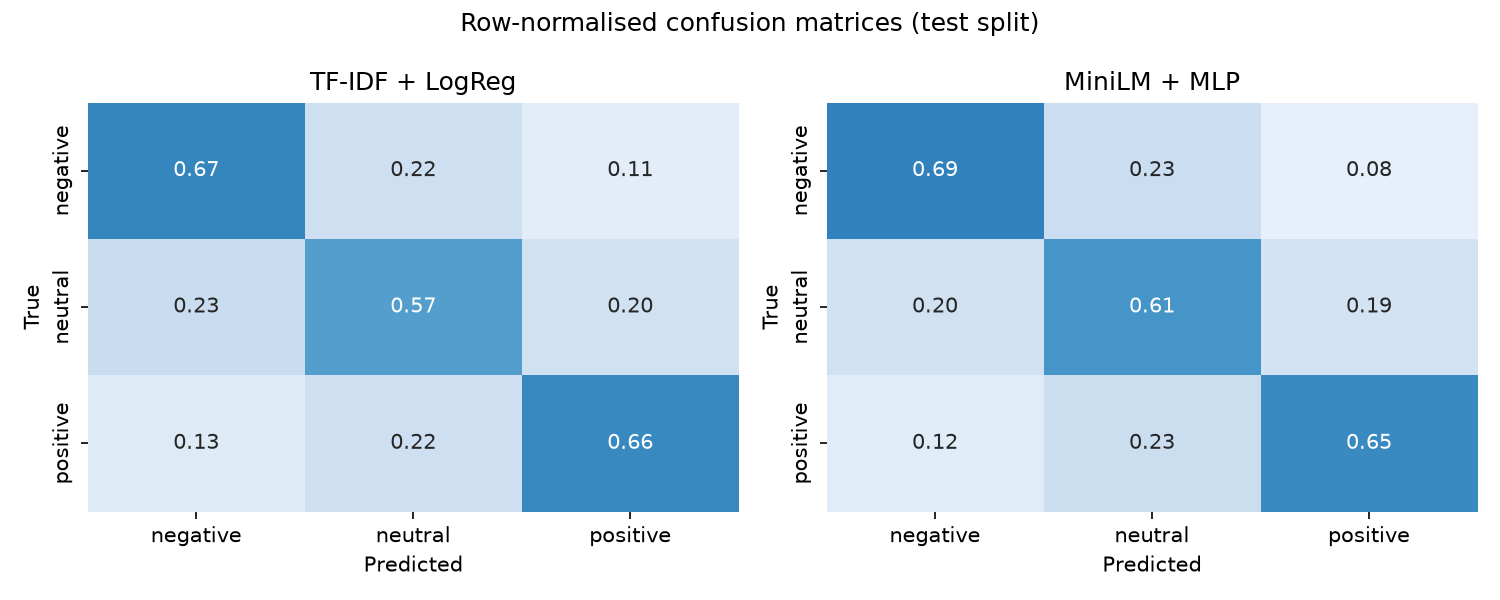
\includegraphics[width=0.85\textwidth]{confusion_matrices.png}
\caption{Row-normalised confusion matrices on the test split. Most errors involve the neutral
class; direct polarity swaps are rare.}
\label{fig:cm}
\end{figure}

\subsection{Bias Check}
\paragraph{Language and code-switching.} Both models are clearly worse on Roman Urdu
(Table~\ref{tab:lang}). The transformer model gains 4 points of macro-F1 over the baseline on
English but \emph{loses} 4 points on Roman Urdu, so its English--Roman Urdu gap (0.136) is more
than twice the baseline's (0.056). Code-switched posts score \emph{higher} than pure Roman
Urdu, because their English words carry sentiment the models already know.

\begin{table}[H]
\centering
\small
\begin{tabular}{lrrrrr}
\toprule
 & & \multicolumn{2}{c}{\textbf{TF-IDF + LogReg}} & \multicolumn{2}{c}{\textbf{MiniLM + MLP}} \\
\cmidrule(lr){3-4}\cmidrule(lr){5-6}
\textbf{Test subgroup} & \textbf{n} & Macro-F1 & AUC & Macro-F1 & AUC \\
\midrule
English (TweetEval)            & 8,981 & 0.629 & 0.816 & \textbf{0.671} & \textbf{0.854} \\
Roman Urdu (all)               & 2,878 & \textbf{0.573} & \textbf{0.770} & 0.535 & 0.723 \\
\quad code-switched            & 147   & \textbf{0.624} & \textbf{0.833} & 0.610 & 0.770 \\
\quad not code-switched        & 2,731 & \textbf{0.569} & \textbf{0.767} & 0.530 & 0.718 \\
\midrule
Gap English $-$ Roman Urdu     &       & 0.056 & 0.045 & 0.136 & 0.131 \\
\bottomrule
\end{tabular}
\caption{Test performance by language subgroup.}
\label{tab:lang}
\end{table}

\paragraph{Gender and race (EEC).} For every EEC sentence the score
$s = P(\text{positive}) - P(\text{negative})$ is computed. Sentences are grouped by (template,
emotion word), the mean female and male scores are compared in each of the 144 groups, and a
paired $t$-test is run over the groups~\cite{eec}. Race uses only the name rows.

\begin{table}[H]
\centering
\small
\resizebox{\textwidth}{!}{%
\begin{tabular}{llrrrr}
\toprule
\textbf{Model} & \textbf{Comparison} & \textbf{Mean gap} & \textbf{\% pairs A$>$B} & \textbf{$p$-value} & \textbf{Accuracy A / B} \\
\midrule
TF-IDF + LogReg & Female $-$ Male            & $+0.070$ & 94.4\% & $5.8\times10^{-11}$ & 0.315 / 0.413 \\
                & Afr.-American $-$ European & $+0.020$ & 97.2\% & $9.9\times10^{-42}$ & 0.281 / 0.351 \\
MiniLM + MLP    & Female $-$ Male            & $-0.034$ & 9.7\%  & $6.4\times10^{-21}$ & 0.939 / 0.920 \\
                & Afr.-American $-$ European & $-0.003$ & 62.5\% & 0.52 (n.s.)         & 0.917 / 0.931 \\
\bottomrule
\end{tabular}}
\caption{EEC Bias Check over 144 (template, emotion word) pairs. A positive gap means group A
receives more positive sentiment.}
\label{tab:bias}
\end{table}

\begin{figure}[H]
\centering
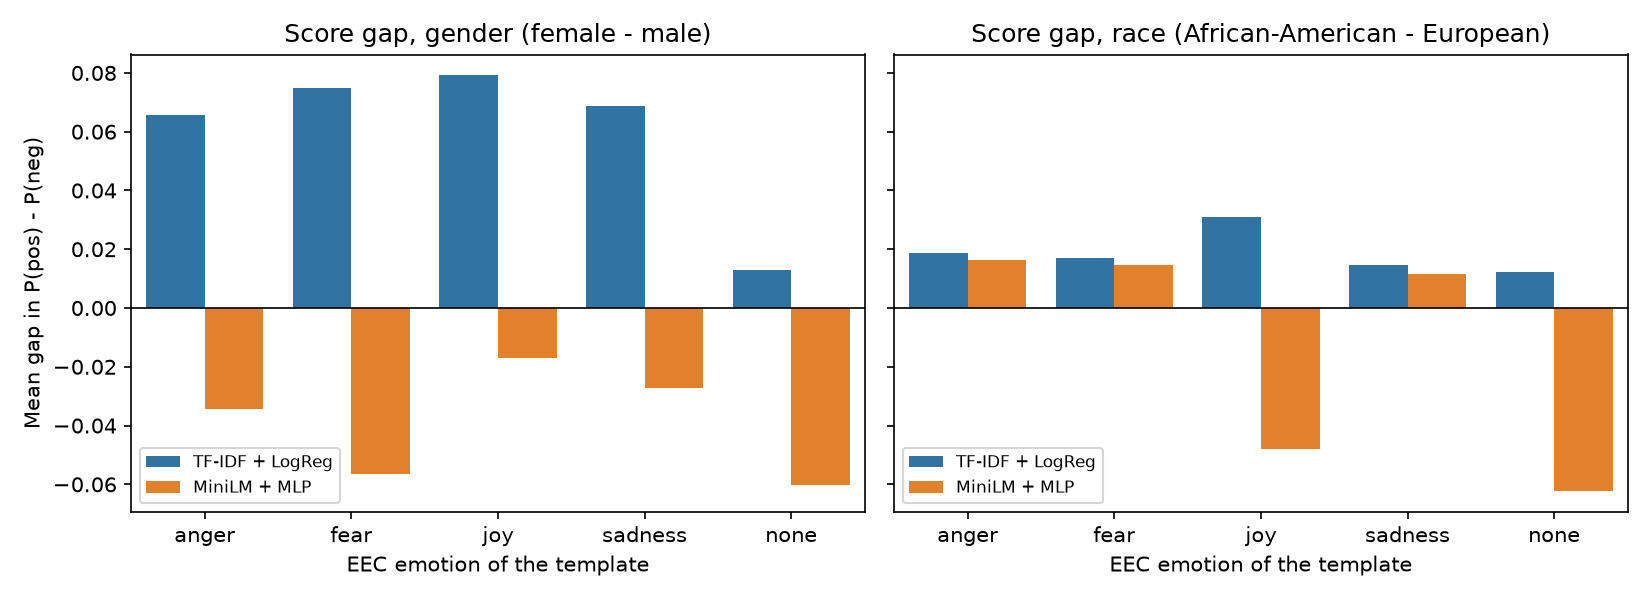
\includegraphics[width=0.95\textwidth]{bias_check.png}
\caption{Mean score gap per EEC emotion. The baseline rates female sentences more positively
for every emotion; the MLP rates them more negatively, most strongly for fear and for the
emotion-free templates.}
\label{fig:bias}
\end{figure}

Both models show a statistically significant gender gap, in opposite directions. The MLP gives
the female version of a sentence a lower score in 90.3\% of pairs; since the encoder is frozen,
this association comes from the pre-trained embeddings. The baseline's gap comes from words it
learned from tweets (e.g.\ positive weight for ``my mom'' and ``her''). On EEC the baseline
reaches only 36.4\% accuracy because 29 of the 40 EEC emotion words are not in its vocabulary,
against 93.0\% for the MLP. The MLP's race gap is not significant ($p = 0.52$). The gender gaps
(0.03--0.07 on a $[-1, 1]$ scale) are much smaller than the language gap, which is the largest
and most harmful bias found.

% ===========================================================================
\section{Phase 5: Research Output}
Phase~5 finalises the comparison with the baselines (\path{src/compare.py}), measures which
components of the architecture matter (\path{src/ablation.py}), applies the mitigation methods
planned in Deliverables~1 and~2 (\path{src/mitigate.py}), shows sample predictions
(\path{src/predict.py}) and discusses why samples fail and what the approach cannot do.

\subsection{Comparative Analysis}
All models are scored on the same held-out test split. Besides the TF-IDF + Logistic
Regression baseline, a \textbf{majority-class} predictor (always ``neutral'') gives a trivial
lower bound. Macro-F1 gets a 95\% bootstrap confidence interval (1,000 resamples of the test
rows)~\cite{bootstrap}. Pairs of models are compared with an exact \textbf{McNemar test} on
per-sample correctness~\cite{dietterich} and a paired bootstrap test on the macro-F1
difference.

\begin{table}[H]
\centering
\footnotesize
\resizebox{\textwidth}{!}{%
\begin{tabular}{lrrrrr}
\toprule
\textbf{Model} & \textbf{Acc.} & \textbf{Macro-F1, all [95\% CI]} & \textbf{English [95\% CI]} & \textbf{Roman Urdu [95\% CI]} & \textbf{AUC} \\
\midrule
Majority class              & 0.454 & 0.208 [0.205, 0.211] & 0.210 [0.206, 0.213] & 0.204 [0.198, 0.209] & 0.500 \\
TF-IDF + LogReg (baseline)  & 0.621 & 0.616 [0.607, 0.624] & 0.628 [0.618, 0.639] & \textbf{0.573} [0.554, 0.590] & 0.806 \\
MiniLM + MLP (ours)         & \textbf{0.643} & \textbf{0.638} [0.629, 0.646] & 0.671 [0.661, 0.681] & 0.535 [0.517, 0.554] & \textbf{0.828} \\
\midrule
MLP + language re-weighting & 0.638 & 0.634 [0.625, 0.642] & 0.666 [0.657, 0.677] & 0.538 [0.520, 0.556] & 0.825 \\
MLP + gender CDA            & 0.638 & 0.632 [0.623, 0.640] & \textbf{0.673} [0.663, 0.683] & 0.503 [0.484, 0.522] & 0.825 \\
MLP + re-weighting + CDA    & 0.638 & 0.631 [0.622, 0.640] & 0.661 [0.651, 0.671] & 0.540 [0.519, 0.559] & 0.822 \\
\bottomrule
\end{tabular}}
\caption{Final comparison on the test split (11,859 rows; 8,981 English, 2,878 Roman Urdu).
The mitigated models are described in Section~\ref{sec:mitigation} (seed-42 models).
Source: \texttt{results/final\_comparison.csv}.}
\label{tab:final}
\end{table}

\begin{table}[H]
\centering
\footnotesize
\resizebox{\textwidth}{!}{%
\begin{tabular}{llrrrr}
\toprule
\textbf{Comparison (A vs.\ B)} & \textbf{Test rows} & \textbf{$\Delta$ macro-F1 [95\% CI]} & \textbf{Bootstrap $p$} & \textbf{Only A / only B correct} & \textbf{McNemar $p$} \\
\midrule
MLP vs.\ TF-IDF + LogReg & All        & $+0.022$ [$+0.012$, $+0.032$] & $<$0.001 & 1,922 / 1,667 & $2.2\times10^{-5}$ \\
                         & English    & $+0.042$ [$+0.031$, $+0.053$] & $<$0.001 & 1,459 / 1,119 & $2.3\times10^{-11}$ \\
                         & Roman Urdu & $-0.038$ [$-0.060$, $-0.016$] & $<$0.001 & 463 / 548     & 0.008 \\
MLP vs.\ majority class  & All        & $+0.429$ [$+0.420$, $+0.439$] & $<$0.001 & 4,326 / 2,092 & $1.5\times10^{-174}$ \\
\midrule
Re-weighting vs.\ MLP    & Roman Urdu & $+0.003$ [$-0.010$, $+0.016$] & 0.680 & 185 / 193 & 0.72 \\
Gender CDA vs.\ MLP      & Roman Urdu & $-0.032$ [$-0.045$, $-0.019$] & $<$0.001 & 113 / 204 & $3.6\times10^{-7}$ \\
Re-weighting + CDA vs.\ MLP & English & $-0.009$ [$-0.016$, $-0.003$] & 0.006 & 423 / 500 & 0.012 \\
\bottomrule
\end{tabular}}
\caption{Significance tests on the test split (selected rows; all rows in
\texttt{results/significance.csv}).}
\label{tab:sig}
\end{table}

\begin{figure}[H]
\centering
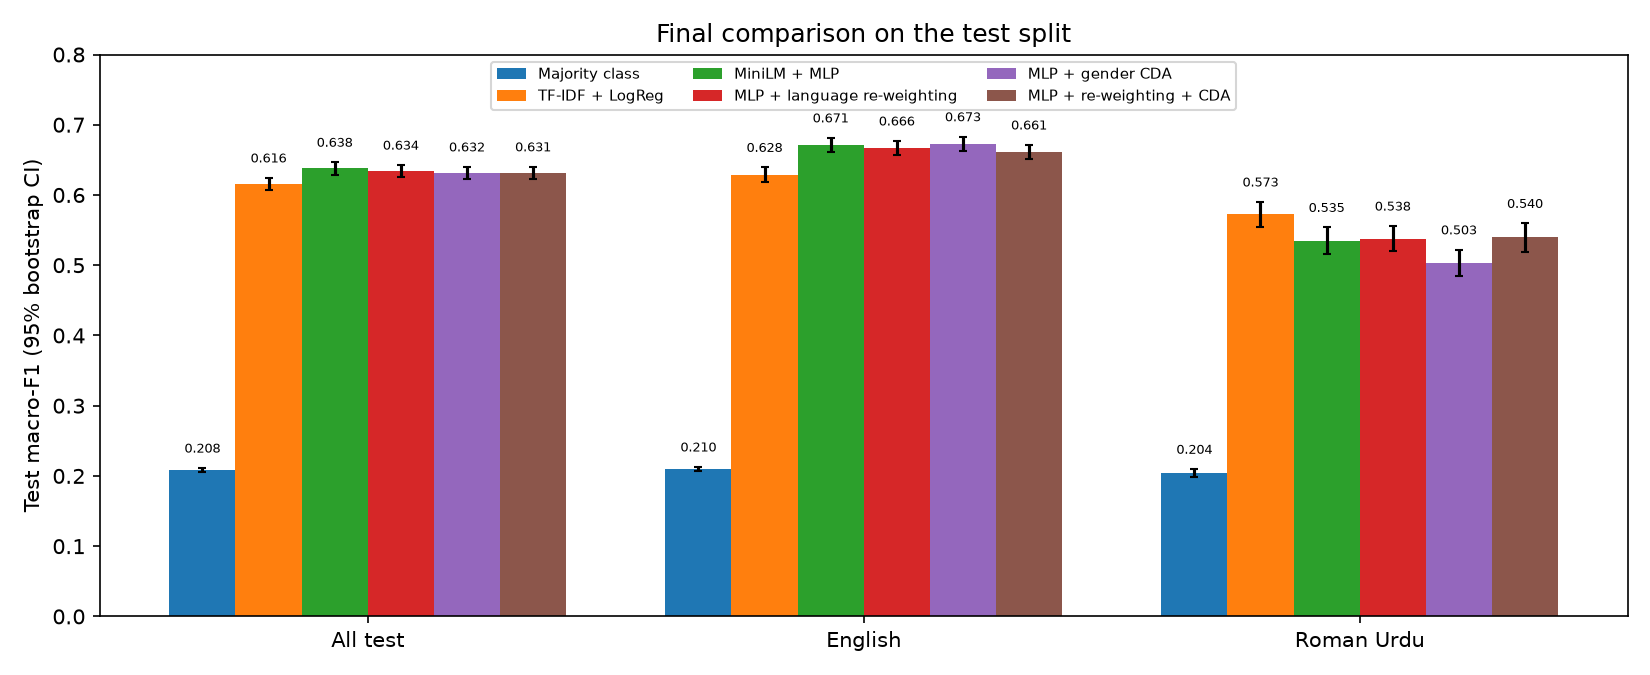
\includegraphics[width=0.98\textwidth]{final_comparison.png}
\caption{Test macro-F1 of every model, overall and per language, with 95\% bootstrap
confidence intervals.}
\label{fig:final}
\end{figure}

\paragraph{Findings.}
\begin{itemize}
  \item Both learned models are far above the majority-class bound (macro-F1 0.21), so the
        task is learnable from these data.
  \item Our MiniLM + MLP model is \textbf{significantly better than the baseline overall}
        ($+0.022$ macro-F1, McNemar $p = 2.2\times10^{-5}$) and \textbf{on English}
        ($+0.042$, $p = 2.3\times10^{-11}$), but \textbf{significantly worse on Roman Urdu}
        ($-0.038$, $p = 0.008$). The confidence intervals of the two languages do not overlap
        for the MLP (0.671 [0.661, 0.681] vs.\ 0.535 [0.517, 0.554]), so the language gap is
        not a sampling artefact.
  \item The overall gain therefore hides a loss for the smaller group. A team that only looks at
        overall macro-F1 or AUC would choose the transformer model and make predictions
        \emph{worse} for Roman Urdu users. This is the central finding of the audit.
\end{itemize}

\subsection{Ablation Study}
\path{src/ablation.py} removes or replaces \emph{one} component of the final model at a time and
retrains the head with all other settings unchanged. Each variant is trained with three seeds
(42, 43, 44); Table~\ref{tab:ablation} reports the mean $\pm$ standard deviation of the test
macro-F1 and the change ($\Delta$) from the full model. The TF-IDF variant feeds the same MLP
with TF-IDF features (baseline settings) reduced to 384 dimensions with truncated SVD and
standardised, so that only the input representation changes.

\begin{table}[H]
\centering
\scriptsize
\setlength{\tabcolsep}{4pt}
\begin{tabular}{lrrrrrrr}
\toprule
 & \multicolumn{2}{c}{\textbf{All test}} & \multicolumn{2}{c}{\textbf{English}} & \multicolumn{2}{c}{\textbf{Roman Urdu}} & \\
\cmidrule(lr){2-3}\cmidrule(lr){4-5}\cmidrule(lr){6-7}
\textbf{Variant} & Macro-F1 & $\Delta$ & Macro-F1 & $\Delta$ & Macro-F1 & $\Delta$ & \textbf{Epochs} \\
\midrule
Full model                     & 0.636 $\pm$ 0.005 & ---      & 0.670 $\pm$ 0.006 & ---      & 0.531 $\pm$ 0.005 & ---      & 11.7 \\
Linear head (no hidden layer)  & 0.598 $\pm$ 0.001 & $-0.038$ & 0.642 $\pm$ 0.001 & $-0.028$ & 0.455 $\pm$ 0.002 & $-0.076$ & 25.3 \\
1 hidden layer                 & 0.634 $\pm$ 0.003 & $-0.002$ & 0.673 $\pm$ 0.002 & $+0.003$ & 0.512 $\pm$ 0.006 & $-0.019$ & 14.0 \\
No dropout                     & 0.634 $\pm$ 0.002 & $-0.002$ & 0.670 $\pm$ 0.003 & $+0.000$ & 0.525 $\pm$ 0.010 & $-0.006$ & 7.3 \\
No class weights               & 0.639 $\pm$ 0.001 & $+0.003$ & 0.674 $\pm$ 0.003 & $+0.004$ & 0.529 $\pm$ 0.004 & $-0.002$ & 8.0 \\
No early stopping (40 epochs)  & 0.616 $\pm$ 0.001 & $-0.021$ & 0.651 $\pm$ 0.002 & $-0.019$ & 0.505 $\pm$ 0.005 & $-0.026$ & 40.0 \\
No Roman Urdu in training      & 0.604 $\pm$ 0.003 & $-0.032$ & 0.675 $\pm$ 0.003 & $+0.005$ & 0.362 $\pm$ 0.016 & $-0.169$ & 11.3 \\
TF-IDF instead of MiniLM       & 0.557 $\pm$ 0.008 & $-0.079$ & 0.565 $\pm$ 0.007 & $-0.105$ & 0.524 $\pm$ 0.020 & $-0.007$ & 6.0 \\
\bottomrule
\end{tabular}
\caption{Ablation study (test split, mean $\pm$ std over 3 seeds). ``Epochs'' is the mean best
epoch. Source: \texttt{results/ablation\_results.csv}.}
\label{tab:ablation}
\end{table}

\begin{figure}[H]
\centering
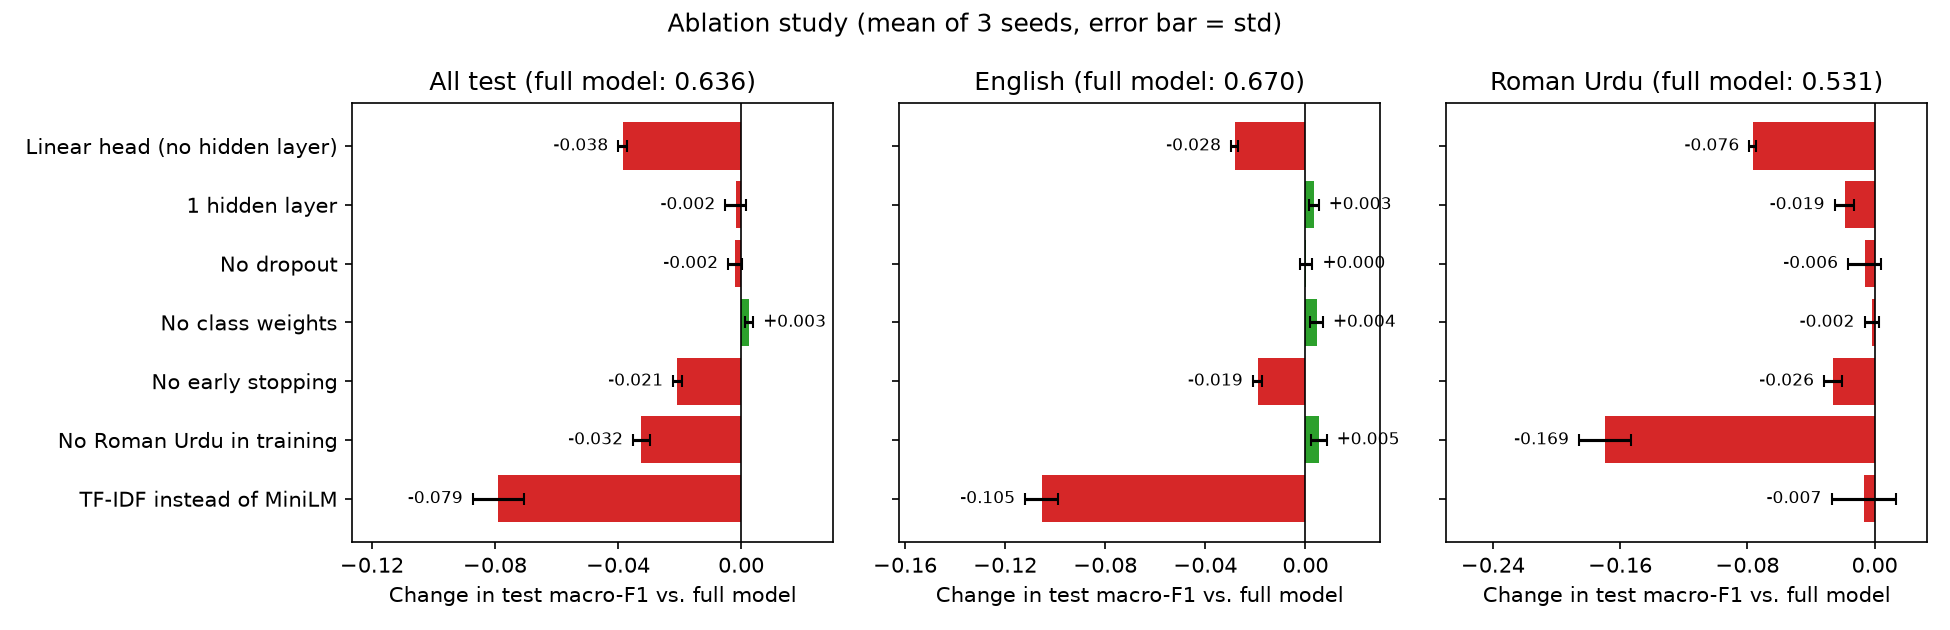
\includegraphics[width=\textwidth]{ablation.png}
\caption{Change in test macro-F1 when one component is removed (mean of 3 seeds, error bar =
standard deviation).}
\label{fig:ablation}
\end{figure}

\paragraph{Which components contribute most.} Ranked by their effect on overall macro-F1:
\begin{enumerate}
  \item \textbf{The pre-trained MiniLM representation} ($-0.079$ when replaced by TF-IDF). Its
        whole contribution is on \textbf{English} ($-0.105$); on Roman Urdu MiniLM features are
        no better than TF-IDF features ($-0.007$, well inside the seed standard deviation of
        0.020). The multilingual pre-training helps the language it has seen a lot of, and
        gives almost nothing for Roman Urdu. This is the direct cause of the language gap.
  \item \textbf{The non-linear head} ($-0.038$ for a linear layer). This is the component that
        matters most for Roman Urdu ($-0.076$): one linear boundary cannot serve two languages
        that share one embedding space. The \emph{second} hidden layer adds nothing overall
        ($-0.002$, within noise) but still helps Roman Urdu ($-0.019$, about three standard
        deviations).
  \item \textbf{Roman Urdu training data} ($-0.032$ overall, $-0.169$ on Roman Urdu). Trained on
        English only, the model reaches only 0.362 on Roman Urdu: there is almost no
        cross-lingual transfer from English tweets to Roman Urdu through the frozen encoder.
        Adding Roman Urdu costs nothing on English ($+0.005$ without it, within noise).
  \item \textbf{Early stopping} ($-0.021$). Training for all 40 epochs overfits (the best epoch
        is 11.7 on average), confirming the training curves in Figure~\ref{fig:curves}.
  \item \textbf{Dropout and class weighting} have no effect beyond seed noise on macro-F1
        ($-0.002$ and $+0.003$). With a frozen 384-d input and early stopping, the head does
        not need extra regularisation, and the imbalance (21/45/34\%) is mild enough that the
        unweighted loss reaches the same macro-F1.
\end{enumerate}

\subsection{Bias Mitigation}
\label{sec:mitigation}
Deliverables~1 and~2 planned mitigation by re-weighting, data augmentation and counterfactual
methods. \path{src/mitigate.py} implements the two that work with a frozen encoder, plus
their combination. Every variant is trained with the tuned hyperparameters and three seeds,
and evaluated on the test split and on the EEC (which stays unseen).
\begin{itemize}
  \item \textbf{Language re-weighting} (targets the language gap). Roman Urdu training rows are
        oversampled with replacement until both languages have the same number of rows
        (41,908 each), so each language contributes equally to the loss.
  \item \textbf{Gender counterfactual data augmentation (CDA)}~\cite{lu2020,zhao2018} (targets
        the gender gap). Every English training sentence containing a gendered word
        (\emph{he/she, his/her, mother/father, mr/mrs}, \ldots; 33 word pairs) is copied with
        the words swapped and the same label. ``Her'' becomes ``his'' before a noun and ``him''
        otherwise. This gives 8,744 copies (e.g.\ ``I hope Milan mom say that she can come
        over'' $\to$ ``I hope Milan dad say that he can come over''), which are embedded with
        the same frozen encoder and added to the training set. No EEC sentence or name is used.
  \item \textbf{Both combined}: CDA, then language re-weighting.
\end{itemize}

\begin{table}[H]
\centering
\footnotesize
\begin{tabular}{lrrrrr}
\toprule
\textbf{Variant} & \textbf{Train rows} & \textbf{Macro-F1} & \textbf{English} & \textbf{Roman Urdu} & \textbf{Language gap} \\
\midrule
Original (Deliverable 2) & 55,339  & \textbf{0.636} & 0.670 & 0.531 $\pm$ 0.005 & 0.139 $\pm$ 0.003 \\
Language re-weighting    & 83,816  & 0.632 & 0.661 & 0.542 $\pm$ 0.004 & 0.120 $\pm$ 0.008 \\
Gender CDA               & 64,083  & 0.633 & \textbf{0.672} & 0.508 $\pm$ 0.012 & 0.164 $\pm$ 0.010 \\
Re-weighting + CDA       & 101,304 & 0.631 & 0.660 & \textbf{0.544} $\pm$ 0.004 & \textbf{0.116} $\pm$ 0.006 \\
\bottomrule
\end{tabular}

\vspace{6pt}
\resizebox{\textwidth}{!}{%
\begin{tabular}{lrrrrrrr}
\toprule
 & \multicolumn{4}{c}{\textbf{Gender gap (female $-$ male)}} & \multicolumn{2}{c}{\textbf{Race gap}} & \\
\cmidrule(lr){2-5}\cmidrule(lr){6-7}
\textbf{Variant} & All rows & Sig. & Names & Noun phr. & Names & Sig. & \textbf{EEC acc.} \\
\midrule
Original (Deliverable 2) & $-0.030$ $\pm$ 0.006 & 3/3 & $-0.038$ & $-0.014$ & $-0.003$ $\pm$ 0.003 & 0/3 & \textbf{0.932} \\
Language re-weighting    & $-0.023$ $\pm$ 0.012 & 3/3 & $-0.025$ & $-0.019$ & $-0.014$ $\pm$ 0.016 & 1/3 & 0.925 \\
Gender CDA               & $-0.038$ $\pm$ 0.018 & 3/3 & $-0.040$ & $-0.033$ & $-0.005$ $\pm$ 0.011 & 2/3 & 0.930 \\
Re-weighting + CDA       & $-0.047$ $\pm$ 0.010 & 3/3 & $-0.046$ & $-0.050$ & $-0.005$ $\pm$ 0.016 & 2/3 & 0.914 \\
\bottomrule
\end{tabular}}
\caption{Mitigation results (mean $\pm$ std over 3 seeds). Top: test macro-F1. Bottom: EEC
score gaps in $P(\text{pos}) - P(\text{neg})$; ``Sig.'' = number of seeds in which the paired
$t$-test gives $p < 0.05$. ``Noun phr.'' = EEC rows that use \emph{she/he, my mother/my father},
etc.\ instead of names. Source: \texttt{results/mitigation\_results.csv}.}
\label{tab:mitigation}
\end{table}

\begin{figure}[H]
\centering
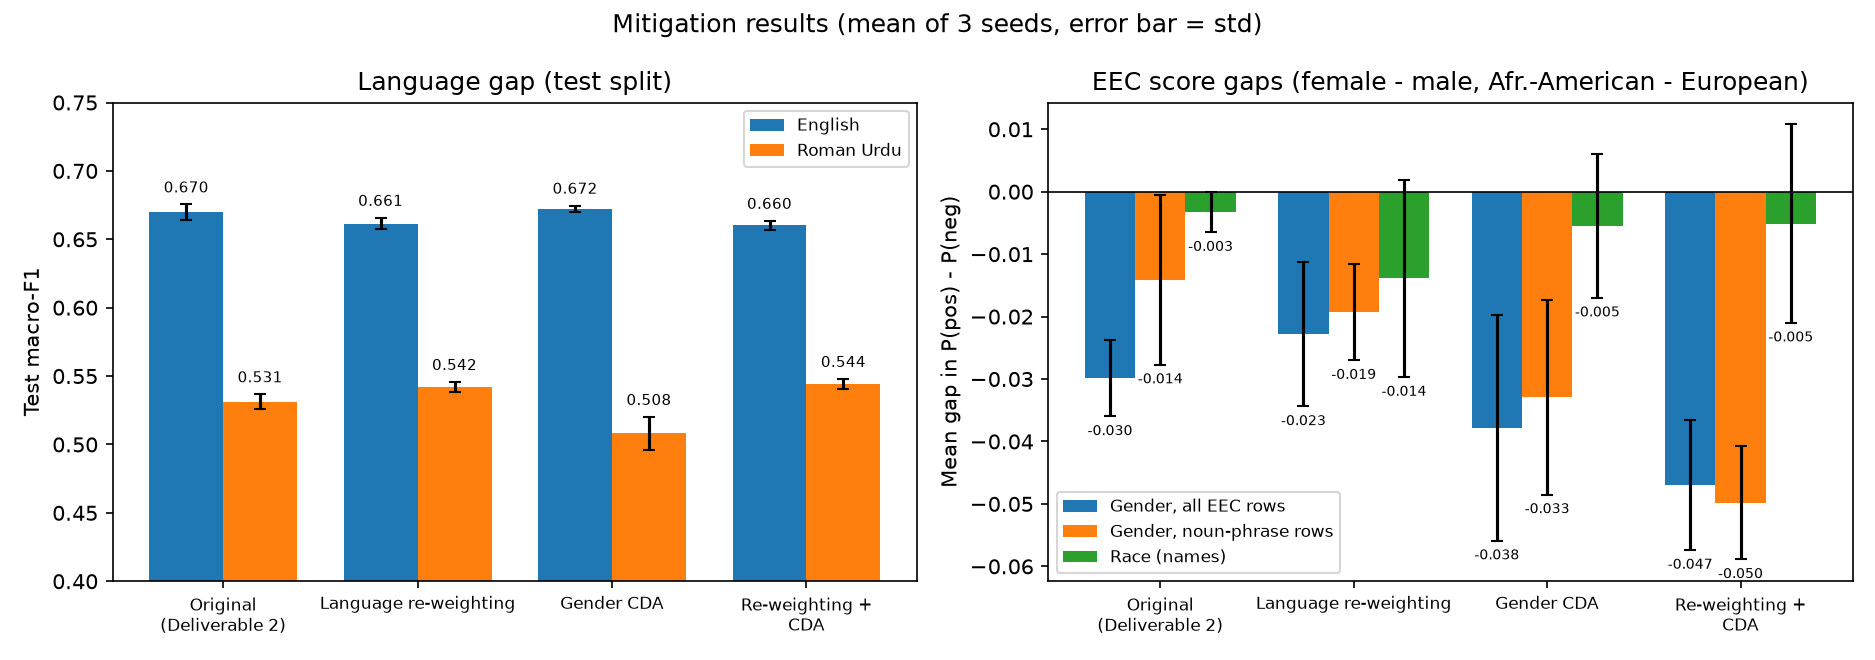
\includegraphics[width=\textwidth]{mitigation.png}
\caption{Effect of the mitigation methods on the language gap (left) and on the EEC score gaps
(right); mean of 3 seeds, error bar = standard deviation.}
\label{fig:mitigation}
\end{figure}

\paragraph{Findings.}
\begin{itemize}
  \item \textbf{Language re-weighting helps, but only a little.} Roman Urdu macro-F1 rises from
        0.531 to 0.542 and the language gap shrinks by 14\% (0.139 $\to$ 0.120). Both changes
        go the same way in all three seeds, but they are small: for the single seed-42 model the
        Roman Urdu gain (+0.003) is not significant ($p = 0.72$, Table~\ref{tab:sig}). The price
        is $-0.009$ on English. Re-weighting changes how much the head listens to Roman Urdu,
        but it cannot add information that the frozen embeddings do not contain (see the
        TF-IDF ablation).
  \item \textbf{Gender CDA did not reduce the gender gap.} The gap stays significant in every
        seed, is larger on average ($-0.038$ vs.\ $-0.030$), and on exactly the noun-phrase
        sentences that CDA swaps it grows in all three seeds ($-0.014 \to -0.033$). CDA also
        lowers Roman Urdu macro-F1 to 0.508, because the extra English rows reduce the Roman
        Urdu share of the training data from 24\% to 21\%. We see two likely reasons for the
        failure. First, the encoder is frozen: the female and male versions of an EEC sentence
        still get different embeddings, and the head, trained on 8,744 swapped tweets, cannot
        remove a gender direction that is entangled with the sentiment information in the
        384-d space. CDA is normally applied when the whole model is trained~\cite{lu2020}.
        Second, word swapping produces imperfect sentences (a male name with ``her'', e.g.\
        ``John Cena wins her 16th title''), so the copies are not clean counterfactuals.
  \item \textbf{The combination shows a trade-off between bias dimensions.} Re-weighting + CDA
        gives the best Roman Urdu score (0.544) and the smallest language gap (0.116), but the
        largest gender gap ($-0.047$) and the lowest EEC accuracy (0.914). Reducing one gap can
        increase another, so all dimensions must be measured together.
  \item \textbf{Variance matters.} The EEC gaps vary noticeably between seeds (std up to 0.018),
        and the race gap of the original model, not significant in the Deliverable~2 run, is
        significant in 1--2 of 3 seeds for the mitigated models. Single-run fairness numbers
        should be read with caution.
\end{itemize}
In short, mitigation applied only to the classification head can narrow the language gap
somewhat but cannot remove it, and simple CDA does not fix the gender gap of a frozen encoder.
The bias sits in the pre-trained representation, so the next step is to adapt the encoder
itself (Section~\ref{sec:limits}).

\subsection{Sample Predictions}
\path{src/predict.py} loads all trained models and predicts any text given on the command line
(\texttt{python src/predict.py "Yeh phone bohat acha hai"}); this is the demo for the final
viva. Figure~\ref{fig:samples} shows its output for twelve sentences written by us, covering
English, Roman Urdu, code-switching, negation, sarcasm and a gender-swapped pair.

\begin{figure}[H]
\centering
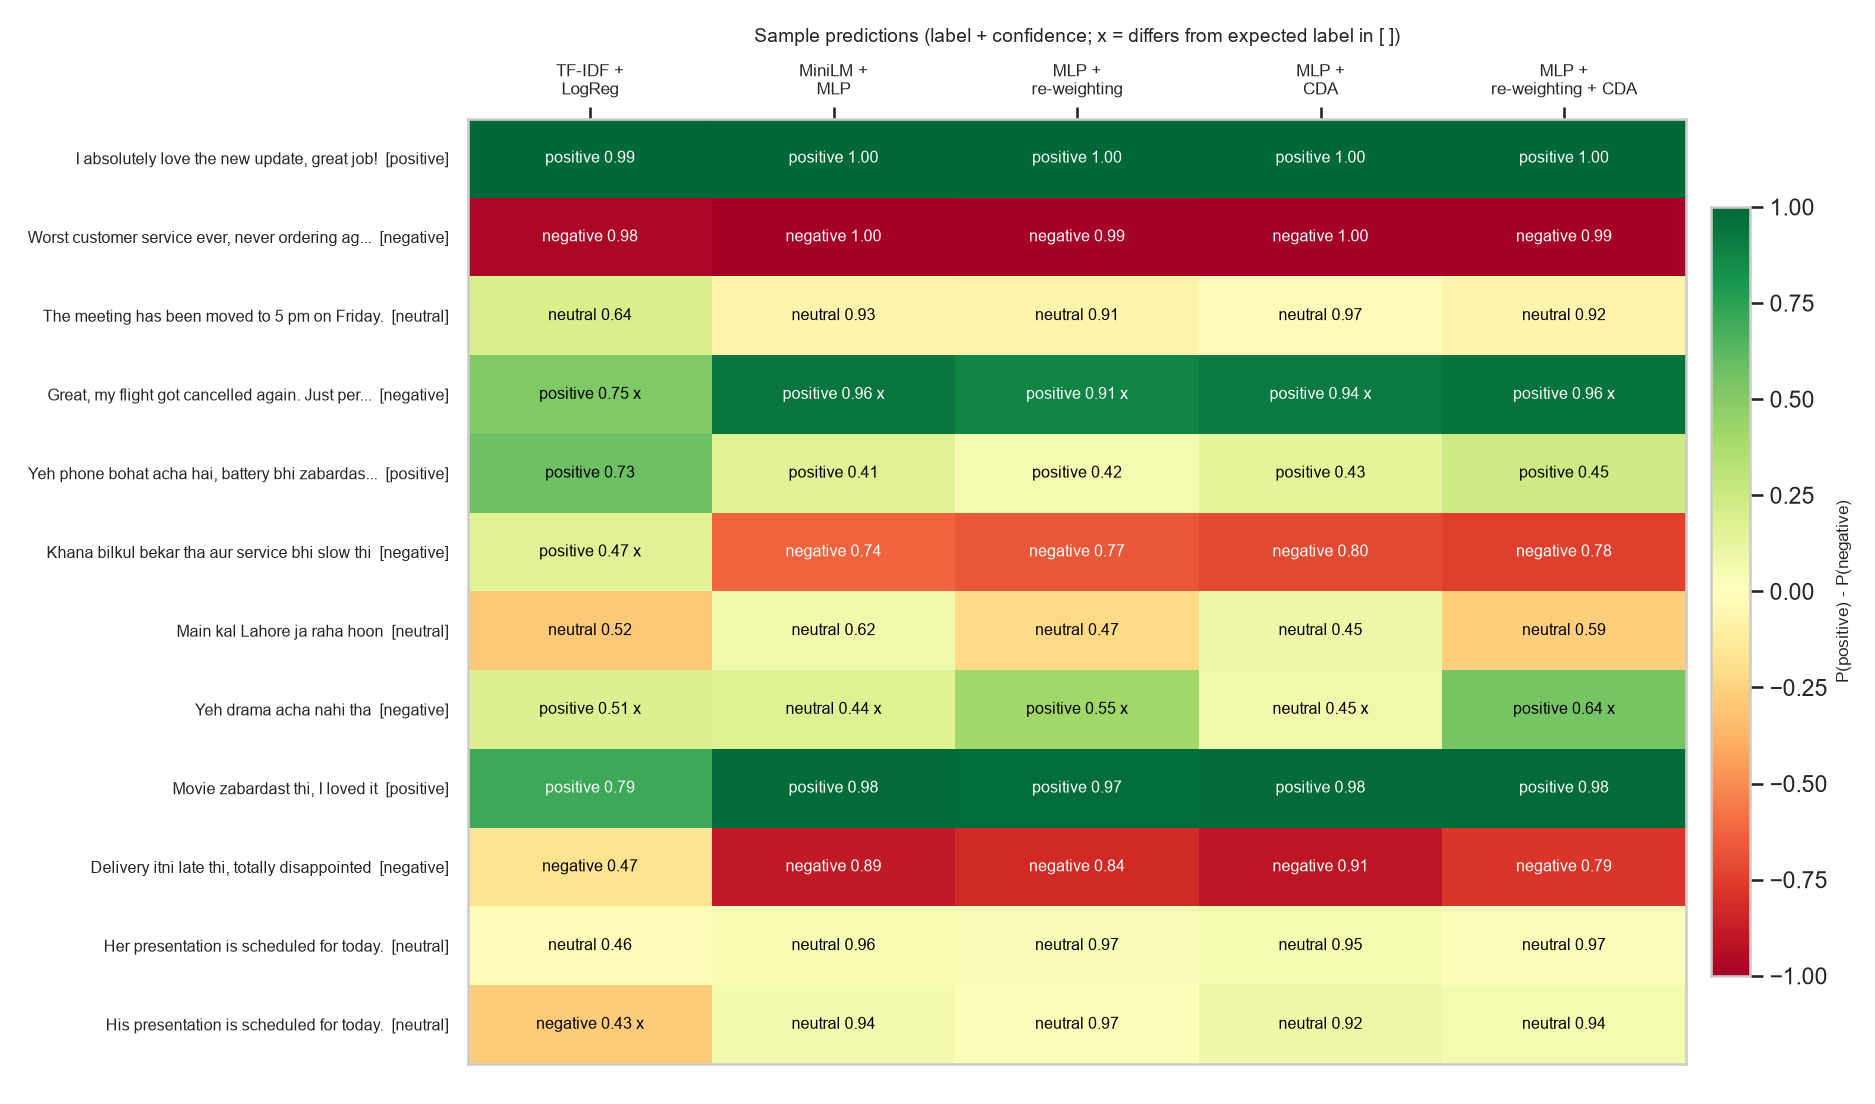
\includegraphics[width=\textwidth]{sample_predictions.png}
\caption{Sample predictions. Each cell gives the predicted label and its probability; the
colour is the score $P(\text{pos}) - P(\text{neg})$; ``x'' marks a prediction that differs
from the expected label in square brackets. Source: \texttt{results/sample\_predictions.csv}.}
\label{fig:samples}
\end{figure}

\noindent The examples show the typical behaviour seen in the test set:
\begin{itemize}
  \item Clear English and code-switched sentences are handled by all models; the MLPs are more
        confident than the baseline.
  \item \textbf{Sarcasm} (``Great, my flight got cancelled again. Just perfect.'') fools every
        model, the MLPs with more than 90\% confidence: the surface words are positive.
  \item \textbf{Roman Urdu negation} (``Yeh drama acha nahi tha'' = this drama was not good) is
        missed by every model: ``acha'' (good) dominates and ``nahi'' (not) is ignored.
  \item The baseline calls ``Khana bilkul bekar tha \ldots'' (the food was totally useless)
        positive, probably because \emph{bilkul} (totally) appears mostly in positive training
        posts (``bilkul sahi'' = absolutely right); the MLPs get it right.
  \item The gender-swapped pair is neutral for every MLP, but the baseline labels the male
        version negative and the female version neutral. Bag-of-words weights on single
        gendered words create exactly the kind of gap measured on the EEC.
\end{itemize}

\subsection{Result Discussion: Why Do Samples Fail?}
\label{sec:why}

\begin{table}[H]
\centering
\footnotesize
\begin{tabular}{lrrr}
\toprule
\textbf{Test slice} & \textbf{n} & \textbf{TF-IDF + LogReg} & \textbf{MiniLM + MLP} \\
\midrule
English, 1--5 tokens              & 92    & 0.272 & 0.359 \\
English, 6--15 tokens             & 2,516 & 0.344 & 0.302 \\
English, $>$15 tokens             & 6,373 & 0.372 & 0.335 \\
English, with negation word       & 1,689 & 0.444 & 0.388 \\
English, no negation word         & 7,292 & 0.345 & 0.311 \\
\midrule
Roman Urdu, 1--5 tokens           & 693   & 0.364 & 0.353 \\
Roman Urdu, 6--15 tokens          & 1,391 & 0.444 & 0.479 \\
Roman Urdu, $>$15 tokens          & 794   & 0.453 & 0.508 \\
Roman Urdu, with negation word    & 354   & 0.486 & 0.511 \\
Roman Urdu, no negation word      & 2,524 & 0.419 & 0.449 \\
Roman Urdu, code-switched         & 147   & 0.360 & 0.388 \\
Roman Urdu, not code-switched     & 2,731 & 0.431 & 0.461 \\
\bottomrule
\end{tabular}
\caption{Error rate (1 $-$ accuracy) by test slice. Negation words: \emph{not, no, never,
n't, \ldots} for English and \emph{nahi, nhi, nahin, na, mat} for Roman Urdu. Source:
\texttt{results/failure\_slices.csv}.}
\label{tab:slices}
\end{table}

\begin{figure}[H]
\centering
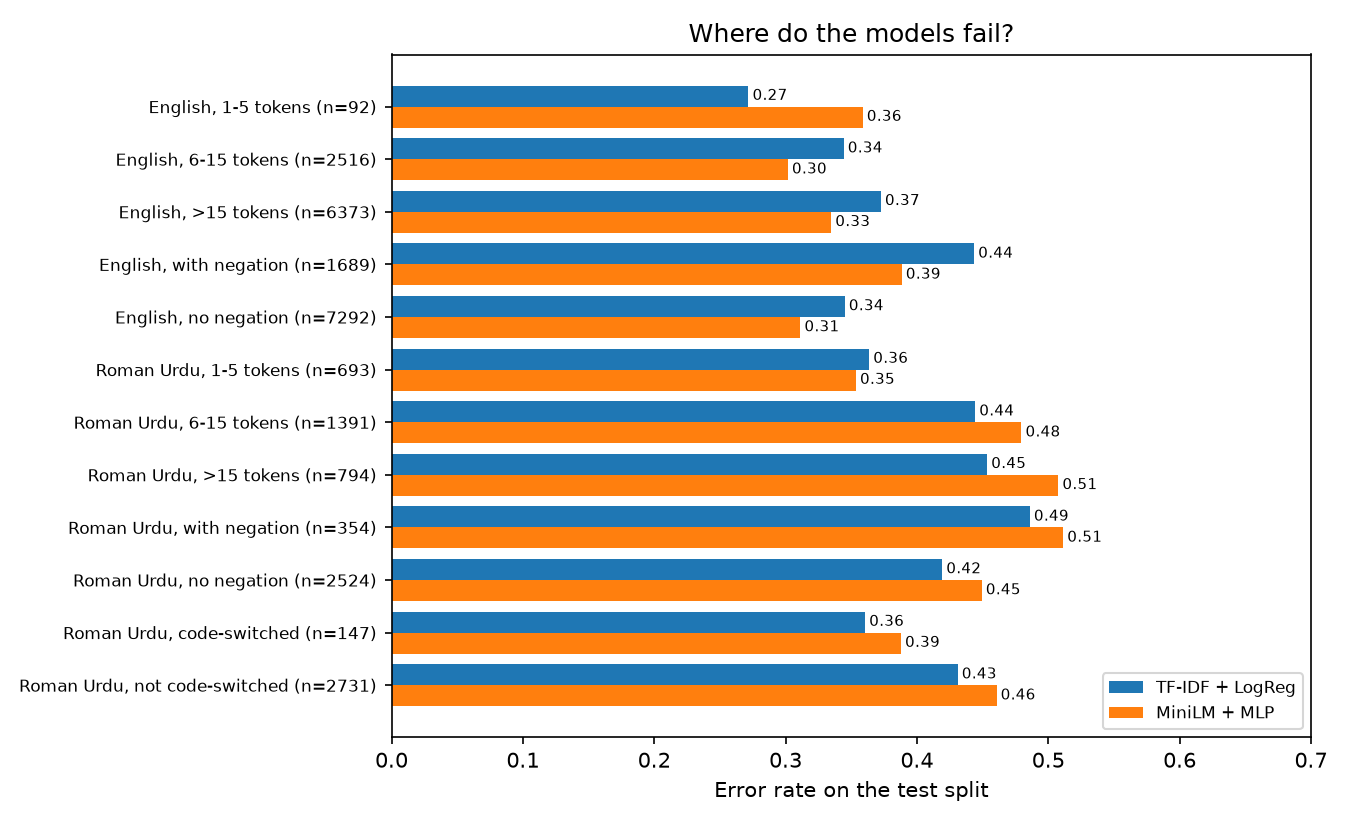
\includegraphics[width=0.8\textwidth]{failure_slices.png}
\caption{Error rate of the two main models on slices of the test split.}
\label{fig:slices}
\end{figure}

\paragraph{1. The neutral class is the hardest.} For the MLP, the four most frequent error types
all involve neutral (neutral$\to$negative 1,088, neutral$\to$positive 1,004,
positive$\to$neutral 919, negative$\to$neutral 559), while direct polarity swaps are rarer
(positive$\to$negative 464, negative$\to$positive 206). Most errors are about \emph{how strong}
the sentiment is, not \emph{which way} it points. The annotators had the same difficulty: 23 of
the 25 conflicting labels in the raw Roman Urdu file (point~6) are neutral vs.\ positive (17) or
neutral vs.\ negative (6), and only 2 are positive vs.\ negative.

\paragraph{2. Roman Urdu fails because of the representation, not the tokenizer.} An obvious
explanation would be that the tokenizer breaks Roman Urdu into many meaningless pieces. That
is not the case: MiniLM's tokenizer produces 1.56 sub-word pieces per word for English test
posts and 1.56 for Roman Urdu (\path{results/failure_stats.json}). The pieces exist, but the
encoder has not learned what they mean in Roman Urdu: its multilingual training data contain
Urdu in Arabic script, so Latin-script Urdu words such as \emph{acha, bekar, zabardast} are most
likely rare in training or read as unrelated English sub-words. The ablation confirms this: MiniLM features are
no better than TF-IDF on Roman Urdu, and there is almost no transfer from English training data.

\paragraph{3. Long Roman Urdu posts fail more often.} The MLP's Roman Urdu error rate rises
from 0.35 (1--5 tokens) to 0.51 ($>$15 tokens), while for English it stays flat or falls. A likely
reason is that long Roman Urdu comments can contain several clauses with different opinions
(e.g.\ ``product is amazing \ldots\ lkn bazar ke lehaz se price zyada hai'' = \emph{but the
price is high compared with the market}, labelled neutral, which both models call positive with
more than 95\% confidence). Mean pooling averages all token vectors into one embedding, so the
deciding clause is diluted by the rest, and with weak Roman Urdu token vectors there is little
left to classify. Very short Roman Urdu posts (``bilkul sahi'') are easier
because one known word decides the label.

\paragraph{4. Negation is a weak point in both languages.} Posts with a negation word have a
higher error rate for both models and both languages (MLP: 0.39 vs.\ 0.31 for English, 0.51
vs.\ 0.45 for Roman Urdu). The encoder was trained for paraphrase similarity, where ``good'' and
``not good'' share most of their words and topic, so the sentence embeddings place them close
together.

\paragraph{5. Sarcasm and world knowledge.} Tweets such as ``\#ThankYouObama for creating the
strongest @user \ldots'' (labelled negative) and the sarcastic flight example in
Figure~\ref{fig:samples} need context that is not in the text.

\paragraph{6. Label noise sets a ceiling for Roman Urdu.} Of the 284 texts that appear more than
once in the raw Roman Urdu file, 25 (8.8\%) carry \emph{different} labels, e.g.\ ``Bilkul
sahi'' and ``Haha'' as both neutral and positive. Cleaning kept only the first copy, but the same
inconsistency exists among non-duplicated texts. The most confident MLP errors in Deliverable~2
were of this kind (``She is awesome'' labelled neutral, predicted positive with 99\%
confidence). Part of the Roman Urdu error is therefore annotation noise that no model can fix.

\subsection{Limitations of the Approach}
\label{sec:limits}
\begin{enumerate}
  \item \textbf{Frozen encoder.} Freezing MiniLM made tuning, ablation and mitigation feasible on
        a CPU-only laptop, but it is also the main limit: the language gap and the gender gap
        both come from the pre-trained representation, and head-level methods could only
        narrow them. Fine-tuning the 118M-parameter encoder on Roman Urdu (and with CDA) was
        not feasible on our hardware and is the most important next step.
  \item \textbf{Sentence embeddings from paraphrase training.} Mean-pooled embeddings trained
        for paraphrase similarity capture topic better than polarity, which explains the
        weakness on negation and sarcasm. A model fine-tuned for sentiment would avoid this.
  \item \textbf{Language and domain are confounded.} All English data are tweets (TweetEval) and
        all Roman Urdu data are comments from a different source with its own annotators. Part
        of the ``language gap'' may be a domain or annotation gap, which we cannot separate
        with the available data.
  \item \textbf{Limited bias evaluation data.} The EEC is English-only and uses American names;
        it cannot measure gender bias for Pakistani names or in Roman Urdu. The code-switched
        test subset is small (147 rows) and is found with a lexicon heuristic.
  \item \textbf{Statistical scope.} Results come from one fixed split and three seeds, and the
        many significance tests are not corrected for multiple comparisons; small effects
        ($|\Delta| < 0.01$) should be read as tendencies.
\end{enumerate}

% ===========================================================================
\section{Conclusion and Future Work}
SentiBias Audit built a complete, reproducible pipeline for auditing a multilingual sentiment
model on English, Roman Urdu and code-switched text and on gender- and race-coded names. A
frozen multilingual MiniLM encoder with a trained MLP head is significantly better than a
TF-IDF baseline overall (macro-F1 0.638 vs.\ 0.616) but significantly \emph{worse} for Roman
Urdu (0.535 vs.\ 0.573), more than doubling the language gap. The ablation study shows why: the
pre-trained representation contributes the most on English and nothing on Roman Urdu, where
only Roman Urdu training data and the non-linear head carry the performance. On the EEC the
model shows a small but statistically significant gender gap and no consistent race gap. Head-level
mitigation reduced the language gap by 14\% (re-weighting) but did not remove it, and
counterfactual augmentation did not reduce the gender gap of the frozen encoder; different gaps
can trade off against each other.

Future work follows directly from these results: (1)~fine-tune the encoder on Roman Urdu
(e.g.\ with a GPU), possibly combined with CDA during fine-tuning; (2)~collect a cleaner,
in-domain Roman Urdu test set to separate language from domain effects; (3)~build an EEC-style
template set with Pakistani names and Roman Urdu sentences, so that gender bias can be measured
in the language this project is about.

% ===========================================================================
\section{Contribution Table}
Each module was committed by the member who implemented it; the authors below match the
\texttt{git log} of the repository (\texttt{git shortlog -sn} shows the commits per author).

\begin{table}[H]
\centering
\footnotesize
\begin{tabular}{>{\raggedright\arraybackslash}p{2.2cm}>{\raggedright\arraybackslash}p{3.5cm}>{\raggedright\arraybackslash}p{3.6cm}>{\raggedright\arraybackslash}p{4.6cm}}
\toprule
\textbf{Git author} & \textbf{Deliverable 1} & \textbf{Deliverable 2} & \textbf{Deliverable 3} \\
\midrule
Saad Jahangir &
\path{data_scripts/download_data.py}, README, \path{.gitignore}, \path{requirements.txt} &
\path{src/config.py}, \path{src/split_data.py}, \path{src/embed.py}, \path{src/baseline.py},
README, Deliverable~2 report &
\path{src/mitigate.py} (language re-weighting, gender CDA, 3-seed evaluation), README, final
report \\
\midrule
Talmeez ur Rehman &
\path{data_scripts/clean_data.py}, \path{data_scripts/feature_eda.py} &
\path{src/model.py}, \path{src/train.py}, \path{src/tune.py} &
Ablation options in \path{src/model.py} and \path{src/train.py}, \path{src/ablation.py}
(3-seed ablation study), \path{src/predict.py} (inference and sample predictions) \\
\midrule
Muhammad Yaseen Asif &
EDA figures, Deliverable~1 report &
\path{src/evaluate.py}, \path{src/bias_check.py} &
\path{src/compare.py} (final comparison, bootstrap CIs, McNemar tests, failure slices,
label-noise and tokenizer analysis) \\
\bottomrule
\end{tabular}
\caption{Contribution Table mapping Git commit authors to project modules.}
\label{tab:contrib}
\end{table}

% ===========================================================================
\section{Repository and Reproducibility}
The repository contains \texttt{README.md}, \texttt{requirements.txt}, the Phase~2 scripts in
\path{data_scripts/}, all modelling and research code in \path{src/}, the metric tables in
\path{results/} and the reports with their figures in \path{report/}. Data and model weights are
not stored in Git: the data are re-downloaded by \path{download_data.py} and the five weight
files are linked from the README (the frozen encoder is downloaded from Hugging Face). All
training uses the fixed seed 42 (plus 43 and 44 for the ablation and mitigation runs) and is
deterministic on CPU. To reproduce every number in this report:
{\small
\begin{verbatim}
pip install -r requirements.txt
python data_scripts/download_data.py && python data_scripts/clean_data.py
python data_scripts/feature_eda.py
python src/split_data.py && python src/embed.py && python src/tune.py
python src/train.py && python src/baseline.py
python src/evaluate.py && python src/bias_check.py
python src/ablation.py && python src/mitigate.py
python src/compare.py && python src/predict.py
\end{verbatim}}

\begin{thebibliography}{99}
\bibitem{uci} Sharf, Z. and Rahman, S. U. (2018). \emph{Roman Urdu Data Set}. UCI Machine
  Learning Repository, dataset 458. \url{https://archive.ics.uci.edu/dataset/458/roman+urdu+data+set}
\bibitem{tweeteval} Barbieri, F., Camacho-Collados, J., Espinosa-Anke, L. and Neves, L. (2020).
  TweetEval: Unified Benchmark and Comparative Evaluation for Tweet Classification.
  In \emph{Findings of EMNLP 2020}, pp.\ 1644--1650.
\bibitem{eec} Kiritchenko, S. and Mohammad, S. M. (2018). Examining Gender and Race Bias in Two
  Hundred Sentiment Analysis Systems. In \emph{Proceedings of the Seventh Joint Conference on
  Lexical and Computational Semantics (*SEM 2018)}, pp.\ 43--53.
\bibitem{sbert} Reimers, N. and Gurevych, I. (2019). Sentence-BERT: Sentence Embeddings using
  Siamese BERT-Networks. In \emph{Proceedings of EMNLP-IJCNLP 2019}, pp.\ 3982--3992.
\bibitem{sbertmulti} Reimers, N. and Gurevych, I. (2020). Making Monolingual Sentence
  Embeddings Multilingual using Knowledge Distillation. In \emph{Proceedings of EMNLP 2020},
  pp.\ 4512--4525.
\bibitem{minilm} Wang, W., Wei, F., Dong, L., Bao, H., Yang, N. and Zhou, M. (2020). MiniLM:
  Deep Self-Attention Distillation for Task-Agnostic Compression of Pre-Trained Transformers.
  In \emph{Advances in Neural Information Processing Systems 33 (NeurIPS 2020)}.
\bibitem{pytorch} Paszke, A. et al.\ (2019). PyTorch: An Imperative Style, High-Performance
  Deep Learning Library. In \emph{Advances in Neural Information Processing Systems 32
  (NeurIPS 2019)}.
\bibitem{sklearn} Pedregosa, F. et al.\ (2011). Scikit-learn: Machine Learning in Python.
  \emph{Journal of Machine Learning Research}, 12, 2825--2830.
\bibitem{adamw} Loshchilov, I. and Hutter, F. (2019). Decoupled Weight Decay Regularization.
  In \emph{International Conference on Learning Representations (ICLR 2019)}.
\bibitem{dietterich} Dietterich, T. G. (1998). Approximate Statistical Tests for Comparing
  Supervised Classification Learning Algorithms. \emph{Neural Computation}, 10(7), 1895--1923.
\bibitem{bootstrap} Efron, B. and Tibshirani, R. J. (1993). \emph{An Introduction to the
  Bootstrap}. Chapman \& Hall/CRC.
\bibitem{zhao2018} Zhao, J., Wang, T., Yatskar, M., Ordonez, V. and Chang, K.-W. (2018). Gender
  Bias in Coreference Resolution: Evaluation and Debiasing Methods. In \emph{Proceedings of
  NAACL-HLT 2018}, pp.\ 15--20.
\bibitem{lu2020} Lu, K., Mardziel, P., Wu, F., Amancharla, P. and Datta, A. (2020). Gender Bias
  in Neural Natural Language Processing. In \emph{Logic, Language, and Security}, Lecture Notes
  in Computer Science 12300, pp.\ 189--202. Springer.
\end{thebibliography}

\end{document}
